\documentclass[11pt]{article}
\newcommand{\DOCFOOT}{AMPERE POINT — automatyzacje w aplikacji Tuya}
\usepackage{fontspec}
\setmainfont{DejaVu Sans}[Scale=0.86]
\setsansfont{DejaVu Sans}[Scale=0.86]
\usepackage[a4paper,top=2.0cm,bottom=1.8cm,left=1.9cm,right=1.9cm]{geometry}
\usepackage{graphicx}
\usepackage{xcolor}
\usepackage{tikz}
\usetikzlibrary{calc}
\usepackage{enumitem}
\usepackage{fancyhdr}
\usepackage{titlesec}
\usepackage{array}
\usepackage{tabularx}
\usepackage{booktabs}
\usepackage[hidelinks]{hyperref}
\hypersetup{pdfauthor={Dawid Cekała — Ampere Point}, pdfcreator={Ampere Point}}
\usepackage{needspace}

\definecolor{apnavy}{HTML}{1A1A1A}
\definecolor{apnavy2}{HTML}{4A4A4A}
\definecolor{apink}{HTML}{1C2430}
\definecolor{apmuted}{HTML}{5B6675}
\definecolor{apline}{HTML}{E3E3E3}
\definecolor{apbg}{HTML}{F7F7F7}
\definecolor{apgreen}{HTML}{1F8A4C}
\definecolor{apgreenbg}{HTML}{E7F5EC}
\definecolor{apwarn}{HTML}{B9791B}
\definecolor{apwarnbg}{HTML}{FBF1DE}
\definecolor{apaccent}{HTML}{EC6434}

\setlength{\parindent}{0pt}
\setlength{\parskip}{0.35em}
\renewcommand{\arraystretch}{1.25}

\pagestyle{fancy}\fancyhf{}
\renewcommand{\headrulewidth}{0pt}
\renewcommand{\footrulewidth}{0pt}
\providecommand{\DOCAUTH}{oprac. Dawid Cekała}
\fancyfoot[L]{\footnotesize\color{apmuted}\DOCFOOT{} \textperiodcentered{} \DOCAUTH}
\fancyfoot[R]{\footnotesize\color{apmuted}\thepage}

% --- wordmark (placeholder do czasu otrzymania pliku logo) ---
\newcommand{\apwordmark}[1][1]{
\includegraphics[height=\dimexpr #1\dimexpr 0.86cm\relax\relax]{logo_ap.png}}

% --- pasek tytulowy ---
\newcommand{\apheader}[2]{%
\noindent\begin{tikzpicture}
  \node[anchor=north west, inner sep=0pt] at (0,0) {\apwordmark[1.15]};
\end{tikzpicture}\hfill
\raisebox{0.20cm}{\parbox[t]{9.2cm}{\raggedleft\footnotesize\color{apmuted}#2}}\\[0.25cm]
{\color{apaccent}\rule{\textwidth}{1.8pt}}\\[0.30cm]
{\fontspec{DejaVu Sans}\bfseries\color{apnavy}\LARGE #1}\\[0.15cm]}

% --- krok: numer w kolku ---
\newcommand{\kroknum}[1]{%
\tikz[baseline=(k.base)]{\node[circle, fill=apaccent, text=white, inner sep=0pt, minimum size=6.2mm,
  font=\fontspec{DejaVu Sans}\bfseries\small] (k) {#1};}}

% --- ramka informacyjna ---
\newcommand{\apinfo}[2]{%
\par\vspace{0.15cm}
\noindent\begin{tikzpicture}
\node[draw=apline, fill=apbg, line width=0.7pt, rounded corners=5pt, inner sep=8pt,
      text width=\dimexpr\textwidth-2\fboxsep-14pt\relax, align=left]
 {\small\textbf{\color{apnavy}#1}\par\vspace{2pt}\color{apink}#2};
\end{tikzpicture}\par\vspace{0.15cm}}

\newcommand{\apwarnbox}[2]{%
\par\vspace{0.15cm}
\noindent\begin{tikzpicture}
\node[draw=apwarn!45, fill=apwarnbg, line width=0.7pt, rounded corners=5pt, inner sep=8pt,
      text width=\dimexpr\textwidth-2\fboxsep-14pt\relax, align=left]
 {\small\textbf{\color{apwarn}#1}\par\vspace{2pt}\color{apink}#2};
\end{tikzpicture}\par\vspace{0.15cm}}

\newcommand{\apokbox}[2]{%
\par\vspace{0.15cm}
\noindent\begin{tikzpicture}
\node[draw=apgreen!40, fill=apgreenbg, line width=0.7pt, rounded corners=5pt, inner sep=8pt,
      text width=\dimexpr\textwidth-2\fboxsep-14pt\relax, align=left]
 {\small\textbf{\color{apgreen}#1}\par\vspace{2pt}\color{apink}#2};
\end{tikzpicture}\par\vspace{0.15cm}}

% --- komorka kroku: obrazek + opis ---
% #1 numer, #2 tytul, #3 opis, #4 plik
\newcommand{\krok}[4]{%
\begin{minipage}[t]{0.485\textwidth}
  \vspace{0pt}
  \begin{center}\includegraphics[width=\linewidth, height=7.0cm, keepaspectratio]{#4}\end{center}
  \vspace{0.12cm}
  {\kroknum{#1}\ \textbf{\color{apnavy}#2}}\par\vspace{0.05cm}
  {\small\color{apink}#3}
\end{minipage}}

\newcommand{\krokbezobrazka}[3]{%
\begin{minipage}[t]{0.485\textwidth}
  \vspace{0pt}
  \begin{center}
  
\begin{tikzpicture}
    \node[draw=apline, fill=apbg, line width=0.7pt, rounded corners=5pt, inner sep=6pt,
          minimum height=7.0cm, text width=5.3cm, align=center]
      {\footnotesize\color{apmuted}(brak zrzutu ekranu\\dla tego kroku)};
  \end{tikzpicture}
  \end{center}
  \vspace{0.12cm}
  {\kroknum{#1}\ \textbf{\color{apnavy}#2}}\par\vspace{0.05cm}
  {\small\color{apink}#3}
\end{minipage}}

% --- os czasu doby: #1 etykieta, #2 lista stref blokady "a/b,c/d"
\newcommand{\osczasu}[2]{%
\begin{tikzpicture}[x=0.62cm, y=1cm]
  \fill[apgreenbg, rounded corners=2pt] (0,0) rectangle (24,0.66);
  \foreach \a/\b in {#2}{ \fill[apwarnbg] (\a,0) rectangle (\b,0.66);
      \draw[apwarn, line width=0.8pt] (\a,0) rectangle (\b,0.66);}
  \draw[apline, line width=0.8pt, rounded corners=2pt] (0,0) rectangle (24,0.66);
  \foreach \h in {0,2,...,24}{ \draw[apline, line width=0.5pt] (\h,0) -- (\h,-0.08);
     \node[below, font=\tiny\color{apmuted}] at (\h,-0.06) {\h};}
  \node[left, font=\small\bfseries\color{apnavy}] at (-0.35,0.33) {#1};
\end{tikzpicture}}

\graphicspath{{screeny/norm/}}

\begin{document}

\apheader{Automatyzacje w aplikacji Tuya}{Jak działają harmonogram i sceny\\ Przykład: sterowanie godzinami ładowania\\ ładowarki AMPERE POINT z Wi-Fi}

{\large\color{apink} Aplikacja daje dwa różne narzędzia do sterowania ładowarką: harmonogram i automatyzacje. Wyglądają podobnie, ale działają zupełnie inaczej i rozwiązują inne problemy. Ten poradnik wyjaśnia, czym się różnią, kiedy użyć którego i jak zbudować własną regułę.}

\vspace{0.35cm}
{\fontspec{DejaVu Sans}\bfseries\color{apnavy}\large Dwa narzędzia, dwie różne zasady działania}

\vspace{0.2cm}
\begin{tabularx}{\textwidth}{@{}p{3.4cm}XX@{}}
\toprule
 & \textbf{\color{apnavy}Harmonogram} & \textbf{\color{apnavy}Automatyzacja (scena)}\\
\midrule
Gdzie się znajduje & W ustawieniach samego urządzenia & W zakładce Smart $\rightarrow$ Automatyzacja\\
Kiedy działa & O wyznaczonej godzinie & Gdy zajdzie określone zdarzenie\\
Co potrafi & Włączyć lub wyłączyć o danej porze & Zareagować na zmianę stanu urządzenia\\
Czego nie potrafi & Reagować na to, co dzieje się pomiędzy godzinami & Zadziałać samoistnie, bez zdarzenia\\
Typowe zastosowanie & „Codziennie o 22:00 włącz” & „Jeśli zacznie ładować w złej porze — przerwij”\\
\bottomrule
\end{tabularx}

\apinfo{Najważniejsza różnica}{Harmonogram wysyła pojedyncze polecenie o wyznaczonej godzinie i na tym kończy się jego rola. Automatyzacja czeka na zdarzenie — sama z siebie nic nie zrobi, ale gdy zdarzenie nastąpi, zareaguje natychmiast. Dlatego w praktyce najczęściej używa się obu naraz.}

\vspace{0.35cm}
{\fontspec{DejaVu Sans}\bfseries\color{apnavy}\large Problem, który to ilustruje}

Załóżmy, że ładowarka ma nie ładować między 19:00 a 22:00. W harmonogramie ustawiamy: o 19:00 wyłącz, o 22:00 włącz. Wygląda poprawnie — i działa, dopóki samochód stoi podłączony przez cały ten czas.

Jeżeli jednak kierowca wróci o 19:10 i dopiero wtedy wepnie wtyczkę, ładowanie ruszy. Polecenie „wyłącz” zostało już wysłane kwadrans wcześniej, a podłączenie samochodu jest dla ładowarki nowym zdarzeniem, które uruchamia ładowanie. Kolejne polecenie z harmonogramu przyjdzie dopiero o 22:00.

Harmonogram nie potrafi tego wychwycić, ponieważ nie obserwuje urządzenia — działa wyłącznie o wyznaczonych godzinach. Potrzebna jest reguła, która patrzy na urządzenie \emph{cały czas}. To właśnie robi automatyzacja.

\clearpage

% ==================== BUDOWA ====================
\apheader{Z czego składa się automatyzacja}{Trzy elementy: warunek, działanie, ograniczenie czasowe}

Każda automatyzacja w aplikacji Tuya ma tę samą budowę. Zrozumienie tych trzech elementów wystarczy, aby tworzyć własne reguły.

\vspace{0.3cm}
\begin{tabularx}{\textwidth}{@{}p{2.7cm}p{3.9cm}X@{}}
\toprule
& \textbf{\color{apnavy}Element} & \textbf{\color{apnavy}Znaczenie}\\
\midrule
If & Warunek (wyzwalacz) & Zdarzenie, które uruchamia regułę. Reguła „śpi”, dopóki to zdarzenie nie nastąpi.\\
Then & Działanie & Co ma się wykonać, gdy warunek zostanie spełniony.\\
Precondition & Ograniczenie czasowe & Ramy, w których reguła w ogóle może zadziałać: godziny, dni tygodnia. Poza nimi reguła jest nieaktywna.\\
\bottomrule
\end{tabularx}

\apwarnbox{Precondition nie jest wyzwalaczem}{To częste nieporozumienie. Ustawienie przedziału 19:00--22:00 nie oznacza „zrób coś o 19:00”. Oznacza „reaguj tylko wtedy, gdy zegar wskazuje między 19:00 a 22:00”. Bez zdarzenia opisanego w sekcji If nic się nie wydarzy.}

\vspace{0.35cm}
{\fontspec{DejaVu Sans}\bfseries\color{apnavy}\large Jakie warunki oferuje ładowarka}

Po wybraniu wyzwalacza When device status changes i wskazaniu ładowarki aplikacja pokazuje listę parametrów, które można obserwować. Najbardziej przydatny jest Work State — stan pracy urządzenia.

\vspace{0.3cm}
\begin{minipage}[t]{0.45\textwidth}
\vspace{0pt}
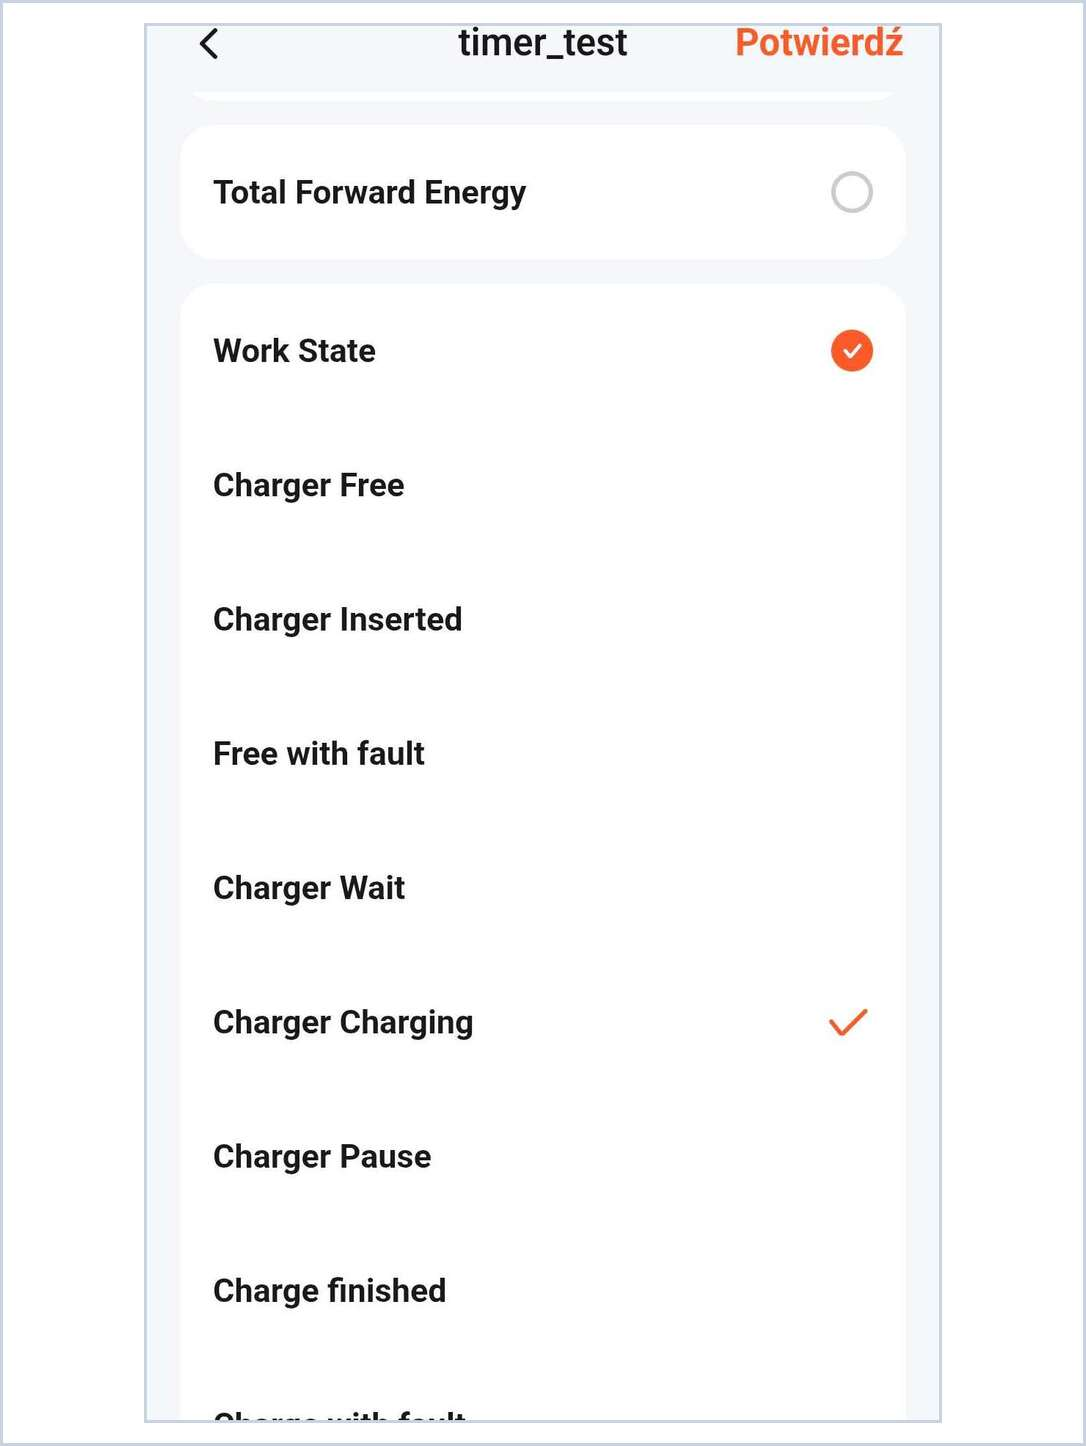
\includegraphics[width=0.84\linewidth]{s05_workstate_charging.jpg}
\end{minipage}
\hfill
\begin{minipage}[t]{0.51\textwidth}
\vspace{0pt}
\small
\begin{tabularx}{\linewidth}{@{}p{3.2cm}X@{}}
\toprule
\textbf{\color{apnavy}Stan} & \textbf{\color{apnavy}Znaczenie}\\
\midrule
Charger Free & Wolna, nic niepodłączone\\
Charger Inserted & Wtyczka włożona do samochodu\\
Charger Wait & Oczekuje na rozpoczęcie\\
Charger Charging & Trwa ładowanie\\
Charger Pause & Ładowanie wstrzymane\\
Charge finished & Ładowanie zakończone\\
Free with fault & Usterka bez podłączonego auta\\
Charge with fault & Usterka w trakcie ładowania\\
\bottomrule
\end{tabularx}
\par\vspace{0.25cm}
Każdy z tych stanów może być wyzwalaczem. Reguła zadziała w chwili, gdy ładowarka \emph{przejdzie} w wybrany stan — a nie wtedy, gdy w nim trwa.
\end{minipage}

\clearpage

% ==================== PRZYKLAD ====================
\apheader{Przykład praktyczny}{Reguła: „nie ładuj w godzinach droższego prądu”\\ budowa krok po kroku}

Zbudujemy regułę przerywającą ładowanie rozpoczęte w godzinach 19:00--22:00 od poniedziałku do piątku. Ta sama ścieżka obowiązuje dla każdej innej reguły — zmieniają się tylko wybrane wartości.

\vspace{0.2cm}

\krok{1}{Utwórz nową automatyzację}{Zakładka Smart $\rightarrow$ Automatyzacja $\rightarrow$ Create. Jeśli masz już inne reguły, użyj przycisku + w prawym górnym rogu.}{s01_automatyzacja_pusta.jpg}
\hfill
\krok{2}{Wybierz rodzaj wyzwalacza}{Lista zawiera kilka typów. When device status changes reaguje na urządzenie. Harmonogram wyzwala o godzinie — przydatny, gdy chcesz zbudować harmonogram w formie sceny.}{s02_wybor_wyzwalacza.jpg}

\vspace{0.42cm}

\krok{3}{Wskaż urządzenie}{Select a single device wybiera jedno urządzenie. Select multiple devices pozwala objąć regułą kilka ładowarek naraz — przydatne przy większej liczbie stanowisk.}{s03_device_single_warunek.jpg}
\hfill
\krok{4}{Wybierz ładowarkę z listy}{Lista pokazuje wszystkie urządzenia w koncie. Urządzenia oznaczone jako \emph{Poza siecią} są w tym momencie niedostępne, ale można ich użyć w regule.}{s04_lista_urzadzen_warunek.jpg}

\clearpage
\apheader{Przykład praktyczny}{ciąg dalszy — warunek i działanie}

\krok{5}{Ustaw warunek}{Wybierz Work State, a następnie konkretny stan — tutaj Charger Charging. Reguła zadziała w chwili rozpoczęcia ładowania.}{s05_workstate_charging.jpg}
\hfill
\krok{6}{Warunek widoczny w sekcji If}{Po zatwierdzeniu wracasz do ekranu sceny. Warunek jest już zapisany. Regułę można rozbudować o kolejne warunki przyciskiem +, wybierając na górze, czy mają być spełnione wszystkie, czy dowolny z nich.}{s06_scena_if_gotowy.jpg}

\vspace{0.42cm}

\krok{7}{Dodaj działanie}{Naciśnij + przy sekcji Then. Poza sterowaniem urządzeniem dostępne są też: uruchomienie innej sceny, opóźnienie oraz powiadomienie.}{s07_dodaj_akcje.jpg}
\hfill
\krok{8}{Wskaż urządzenie do sterowania}{Może to być inne urządzenie niż w warunku — na tym polega siła scen. Tutaj sterujemy tą samą ładowarką, więc wybieramy ją ponownie.}{s08_device_single_akcja.jpg}

\clearpage
\apheader{Przykład praktyczny}{ciąg dalszy — ograniczenie czasowe}

\krok{9}{Wybierz ładowarkę}{Ta sama lista urządzeń co poprzednio.}{s09_lista_urzadzen_akcja.jpg}
\hfill
\krok{10}{Ustaw parametr do zmiany}{Switch to włączenie i wyłączenie ładowania. Dostępne są również Charge Current Set (ograniczenie prądu) oraz Work Mode — można więc na przykład nie przerywać ładowania, tylko zmniejszyć prąd.}{s10_switch_off.jpg}

\vspace{0.42cm}

\krok{11}{Sprawdź komplet reguły}{Ekran pokazuje warunek, działanie oraz pozycję Precondition, domyślnie ustawioną na \emph{Cały dzień}. Bez jej zmiany reguła działałaby przez całą dobę.}{s11_scena_if_then.jpg}
\hfill
\krok{12}{Otwórz ograniczenie czasowe}{Naciśnij Precondition, a następnie Obowiązywanie odcinka czasu. Pozycja Valid When pozwala dodatkowo uzależnić regułę od stanu innych urządzeń lub od pogody.}{s12_precondition_calydzien.jpg}

\clearpage
\apheader{Przykład praktyczny}{zakończenie — godziny, dni, zapis}

\krok{13}{Wybierz tryb ręczny}{Poza ustawieniem ręcznym dostępne są tryby Dzień i Noc, liczone od wschodu i zachodu słońca — przydatne np. do oświetlenia. Dla stałych godzin wybierz Dostosowane.}{s13_czas_calydzien.jpg}
\hfill
\krok{14}{Otwórz wybór godzin}{Po zaznaczeniu trybu ręcznego pojawia się pozycja Okres czasu z domyślną wartością od 00:00 do 23:59.}{s14_czas_dostosowane.jpg}

\vspace{0.42cm}

\krok{15}{Ustaw przedział godzin}{Warto zaczynać przedział kilka minut wcześniej niż godzina graniczna — reguła zaczyna wtedy czuwać, zanim harmonogram wyśle swoje polecenie.}{s15_okres_kola.jpg}
\hfill
\krok{16}{Ustaw dni tygodnia i miasto}{Powtórz to wybór dni. Miasto jest potrzebne aplikacji do prawidłowego liczenia czasu lokalnego oraz godzin wschodu i zachodu słońca.}{s16_czas_gotowy.jpg}

\clearpage
\apheader{Przykład praktyczny}{zakończenie}

\krok{17}{Wskaż miasto na mapie}{Wystarczy przybliżyć okolicę i zatwierdzić przyciskiem OK.}{s17_miasto_mapa.jpg}
\hfill
\krok{18}{Zamknij ustawienia}{Ustawiony przedział widnieje przy pozycji Obowiązywanie odcinka czasu. Naciśnij Zakończ.}{s18_precondition_gotowy.jpg}

\vspace{0.42cm}

\krok{19}{Nazwij regułę}{Dobra nazwa zawiera godziny i efekt działania. Przy kilku regułach oszczędza to sporo czasu — widać wszystko na liście bez wchodzenia w szczegóły.}{s19_nazwa_sceny.jpg}
\hfill
\krok{20}{Sprawdź, czy jest aktywna}{Reguła pojawia się na liście z przełącznikiem. Zielony oznacza aktywną. Regułę można w każdej chwili wyłączyć bez usuwania — przydatne np. na czas urlopu.}{s20_lista_gotowa.jpg}

\clearpage

% ==================== AUTOMATYZACJA WLACZAJACA ====================
\apheader{Automatyzacja, która włącza ładowanie}{Druga reguła: wyzwalacz godzinowy zamiast harmonogramu}

Dotąd budowaliśmy regułę, która ładowanie \emph{przerywa}. Automatyzacja potrafi jednak również je \emph{rozpocząć} — wystarczy zamiast stanu urządzenia wybrać wyzwalacz godzinowy. Taka reguła zastępuje wpis harmonogramu i ma nad nim dwie przewagi.

\vspace{0.25cm}
\begin{tabularx}{\textwidth}{@{}p{5.4cm}X@{}}
\toprule
\textbf{\color{apnavy}Przewaga} & \textbf{\color{apnavy}Na czym polega}\\
\midrule
Ustawia przełącznik & Automatyzacja przestawia główny przełącznik ładowarki, więc uruchamia ładowanie także wtedy, gdy zostało wcześniej wyłączone przez inną regułę.\\
Ustawia prąd osobnym poleceniem & Wartość prądu wysyłana jest jako niezależne polecenie, a nie jako część wpisu harmonogramu.\\
\bottomrule
\end{tabularx}

\apwarnbox{Dlaczego to ma znaczenie}{Wpis harmonogramu włączający ładowanie ustawia tryb pracy urządzenia, ale nie przestawia głównego przełącznika. Jeżeli przełącznik został wcześniej wyłączony — na przykład przez automatyzację blokującą albo przez wpis wyłączający — kolejny wpis harmonogramu nie ma czego uruchomić. Ładowarka ma wtedy podłączony samochód, prawidłowy tryb i prawidłowy prąd, a mimo to nie ładuje. Automatyzacja opisana na tej stronie omija ten problem.}

\vspace{0.3cm}

\krok{1}{Utwórz drugą automatyzację}{Ta sama ścieżka co poprzednio: Smart $\rightarrow$ Automatyzacja $\rightarrow$ przycisk + w prawym górnym rogu.}{s01_automatyzacja_pusta.jpg}
\hfill
\krok{2}{Wybierz wyzwalacz godzinowy}{Tym razem nie \emph{When device status changes}, tylko pozycja harmonogramu — reguła ma zadziałać o wyznaczonej porze, a nie w reakcji na urządzenie.}{s02_wybor_wyzwalacza.jpg}

\clearpage
\apheader{Automatyzacja, która włącza ładowanie}{ciąg dalszy — godzina i pierwsze działanie}

\krokbezobrazka{3}{Ustaw godzinę i dni tygodnia}{Wskaż porę rozpoczęcia ładowania oraz dni, w które reguła ma obowiązywać. Powtarzanie ustaw od razu — bez niego reguła wykona się tylko raz.}
\hfill
\krok{4}{Dodaj pierwsze działanie}{Naciśnij + przy sekcji Then i wybierz sterowanie urządzeniem. Ta reguła będzie miała dwa działania, nie jedno.}{s07_dodaj_akcje.jpg}

\vspace{0.42cm}

\krok{5}{Wskaż ładowarkę}{Ta sama lista urządzeń co przy poprzedniej regule.}{s09_lista_urzadzen_akcja.jpg}
\hfill
\krok{6}{Wybierz Charge Current Set}{Pierwsze działanie ustawia prąd ładowania. Wybierz wartość, z jaką ma pracować ładowarka — na przykład 13 A. To polecenie wysyłane jest niezależnie od nastawy w ustawieniach urządzenia.}{s10_switch_off.jpg}

\clearpage
\apheader{Automatyzacja, która włącza ładowanie}{zakończenie — drugie działanie i zapis}

\krok{7}{Dodaj drugie działanie}{Ponownie naciśnij + przy sekcji Then, wskaż tę samą ładowarkę, wybierz Switch i ustaw wartość na włączony. To ono uruchamia ładowanie.}{s07_dodaj_akcje.jpg}
\hfill
\krokbezobrazka{8}{Sprawdź komplet reguły}{W sekcji Then powinny widnieć dwa działania: ustawienie prądu oraz włączenie. Kolejność ma znaczenie — prąd ustawiamy przed włączeniem.}

\vspace{0.42cm}

\krok{9}{Nazwij regułę}{Nazwa powinna odróżniać ją od reguły blokującej, na przykład „22:00 ładowanie on 13 A”.}{s19_nazwa_sceny.jpg}
\hfill
\krokbezobrazka{10}{Sprawdź obie reguły na liście}{Na liście automatyzacji powinny być teraz dwie pozycje: włączająca i blokująca, obie z aktywnym przełącznikiem.}

\apinfo{Reguła włączająca a reguła blokująca}{Obie mogą pracować razem, ale ich godziny nie powinny się stykać. Jeżeli blokada obowiązuje do 22:00, regułę włączającą ustaw na 22:02. Automatyzacja blokująca reaguje na rozpoczęcie ładowania w ułamku sekundy, więc start dokładnie o godzinie granicznej zostanie przez nią przerwany.}

\clearpage

% ==================== ZASADY ====================
\apheader{Zasady, o których warto pamiętać}{Typowe błędy i sprawdzone rozwiązania}

\vspace{0.1cm}
{\fontspec{DejaVu Sans}\bfseries\color{apnavy}\large Cztery najczęstsze błędy}

\vspace{0.2cm}
\begin{tabularx}{\textwidth}{@{}p{5.0cm}X@{}}
\toprule
\textbf{\color{apnavy}Błąd} & \textbf{\color{apnavy}Skutek i jak go uniknąć}\\
\midrule
Brak zaznaczonych dni w harmonogramie & Wpis wykona się jednorazowo i przestanie działać. Zawsze ustaw powtarzanie.\\
Reguła blokująca użyta do włączania & Reguła reagująca na rozpoczęcie ładowania potrafi je tylko przerwać. Do włączania służy osobna automatyzacja z wyzwalaczem godzinowym.\\
Reguła bez ograniczenia czasowego & Zadziała o każdej porze doby. Ustaw Precondition.\\
Błędna strefa czasowa urządzenia & Wszystkie godziny przesuwają się o kilka godzin. Sprawdź w ustawieniach urządzenia.\\
\bottomrule
\end{tabularx}

\vspace{0.4cm}
{\fontspec{DejaVu Sans}\bfseries\color{apnavy}\large Kiedy harmonogram, a kiedy automatyzacja}

\vspace{0.2cm}
\begin{tabularx}{\textwidth}{@{}p{6.6cm}X@{}}
\toprule
\textbf{\color{apnavy}Potrzeba} & \textbf{\color{apnavy}Narzędzie}\\
\midrule
Rozpocząć ładowanie o stałej porze & Automatyzacja z wyzwalaczem godzinowym\\
Przerwać ładowanie o stałej porze & Harmonogram albo automatyzacja godzinowa\\
Nie dopuścić do ładowania w danych godzinach, niezależnie od pory podłączenia & Automatyzacja z warunkiem \emph{Charger Charging}\\
Zmniejszyć prąd zamiast przerywać & Automatyzacja z działaniem \emph{Charge Current Set}\\
Otrzymać powiadomienie o usterce & Automatyzacja z warunkiem \emph{Charge with fault} i działaniem \emph{Send notification}\\
Sterować kilkoma ładowarkami naraz & Automatyzacja z opcją \emph{Select multiple devices}\\
\bottomrule
\end{tabularx}

\apinfo{Połączenie z internetem}{Harmonogram zapisuje się w samym urządzeniu i po zapisaniu działa również bez internetu. Automatyzacje są wykonywane w chmurze i wymagają połączenia. Po dłuższym zaniku zasilania urządzenie może potrzebować ponownej synchronizacji z aplikacją, aby odtworzyć zapisane godziny. Jeżeli zależy Ci na sterowaniu prądem, wybierz automatyzację — harmonogram nie zawsze przekazuje wartość prądu poprawnie.}

\apokbox{Rozwiązanie najpewniejsze technicznie}{Jeżeli sterowanie godzinami ładowania ma być całkowicie niezawodne, warto ustawić harmonogram również w samym samochodzie. Pojazd nie pobiera wtedy prądu poza wyznaczonymi godzinami niezależnie od aplikacji, ładowarki i połączenia z internetem.}

\vspace{0.5cm}
{\color{apline}\rule{\textwidth}{0.8pt}}\\[0.15cm]
{\footnotesize\color{apmuted} W razie pytań prosimy o kontakt: hello@amperepoint.com}

\end{document}
